% Created by tikzDevice version 0.12 on 2018-09-28 04:16:59
% !TEX encoding = UTF-8 Unicode
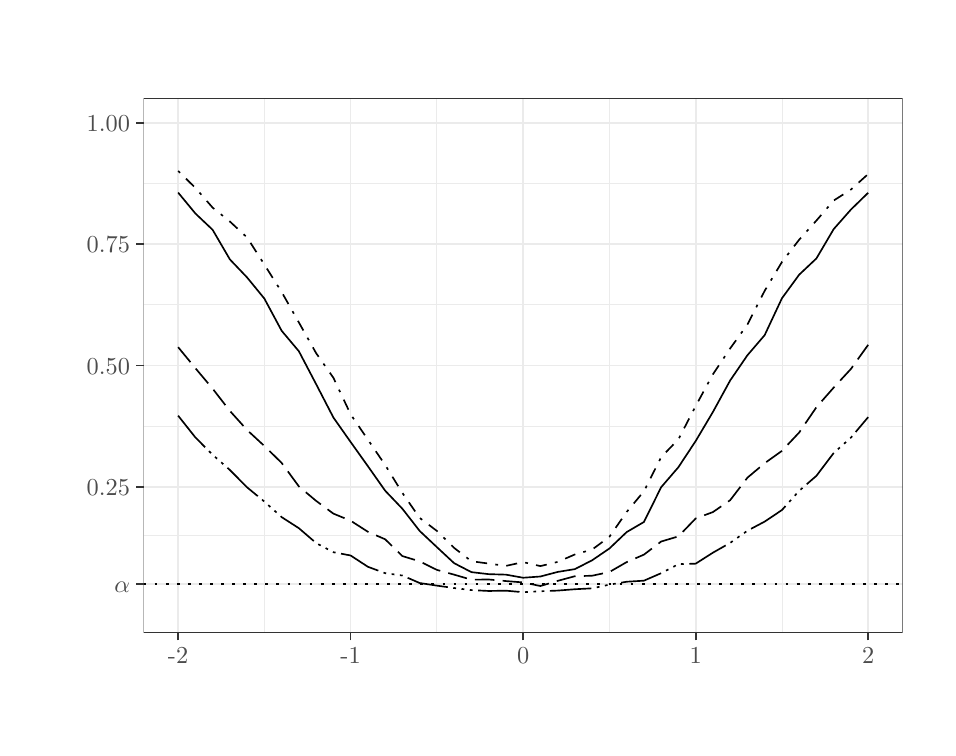
\begin{tikzpicture}[x=1pt,y=1pt]
\definecolor{fillColor}{RGB}{255,255,255}
\path[use as bounding box,fill=fillColor,fill opacity=0.00] (0,0) rectangle (325.21,252.94);
\begin{scope}
\path[clip] (  0.00,  0.00) rectangle (325.21,252.94);
\definecolor{drawColor}{RGB}{255,255,255}
\definecolor{fillColor}{RGB}{255,255,255}

\path[draw=drawColor,line width= 0.6pt,line join=round,line cap=round,fill=fillColor] (  0.00,  0.00) rectangle (325.21,252.94);
\end{scope}
\begin{scope}
\path[clip] ( 41.90, 34.26) rectangle (316.18,227.38);
\definecolor{fillColor}{RGB}{255,255,255}

\path[fill=fillColor] ( 41.90, 34.26) rectangle (316.18,227.38);
\definecolor{drawColor}{gray}{0.92}

\path[draw=drawColor,line width= 0.3pt,line join=round] ( 41.90, 69.37) --
	(316.18, 69.37);

\path[draw=drawColor,line width= 0.3pt,line join=round] ( 41.90,108.87) --
	(316.18,108.87);

\path[draw=drawColor,line width= 0.3pt,line join=round] ( 41.90,152.76) --
	(316.18,152.76);

\path[draw=drawColor,line width= 0.3pt,line join=round] ( 41.90,196.65) --
	(316.18,196.65);

\path[draw=drawColor,line width= 0.3pt,line join=round] ( 85.53, 34.26) --
	( 85.53,227.38);

\path[draw=drawColor,line width= 0.3pt,line join=round] (147.87, 34.26) --
	(147.87,227.38);

\path[draw=drawColor,line width= 0.3pt,line join=round] (210.21, 34.26) --
	(210.21,227.38);

\path[draw=drawColor,line width= 0.3pt,line join=round] (272.55, 34.26) --
	(272.55,227.38);

\path[draw=drawColor,line width= 0.6pt,line join=round] ( 41.90, 51.81) --
	(316.18, 51.81);

\path[draw=drawColor,line width= 0.6pt,line join=round] ( 41.90, 86.93) --
	(316.18, 86.93);

\path[draw=drawColor,line width= 0.6pt,line join=round] ( 41.90,130.82) --
	(316.18,130.82);

\path[draw=drawColor,line width= 0.6pt,line join=round] ( 41.90,174.71) --
	(316.18,174.71);

\path[draw=drawColor,line width= 0.6pt,line join=round] ( 41.90,218.60) --
	(316.18,218.60);

\path[draw=drawColor,line width= 0.6pt,line join=round] ( 54.37, 34.26) --
	( 54.37,227.38);

\path[draw=drawColor,line width= 0.6pt,line join=round] (116.70, 34.26) --
	(116.70,227.38);

\path[draw=drawColor,line width= 0.6pt,line join=round] (179.04, 34.26) --
	(179.04,227.38);

\path[draw=drawColor,line width= 0.6pt,line join=round] (241.38, 34.26) --
	(241.38,227.38);

\path[draw=drawColor,line width= 0.6pt,line join=round] (303.71, 34.26) --
	(303.71,227.38);
\definecolor{drawColor}{RGB}{0,0,0}

\path[draw=drawColor,line width= 0.6pt,dash pattern=on 1pt off 3pt on 4pt off 3pt ,line join=round] ( 54.37,201.18) --
	( 60.60,195.04) --
	( 66.83,187.91) --
	( 73.07,182.89) --
	( 79.30,177.10) --
	( 85.53,167.33) --
	( 91.77,157.43) --
	( 98.00,146.41) --
	(104.24,135.31) --
	(110.47,126.43) --
	(116.70,113.23) --
	(122.94,104.06) --
	(129.17, 94.93) --
	(135.40, 84.82) --
	(141.64, 75.80) --
	(147.87, 71.09) --
	(154.10, 64.95) --
	(160.34, 60.14) --
	(166.57, 59.29) --
	(172.81, 58.45) --
	(179.04, 59.82) --
	(185.27, 58.38) --
	(191.51, 59.89) --
	(197.74, 62.59) --
	(203.97, 64.35) --
	(210.21, 68.98) --
	(216.44, 77.94) --
	(222.68, 85.42) --
	(228.91, 97.74) --
	(235.14,104.20) --
	(241.38,116.21) --
	(247.61,127.69) --
	(253.84,137.03) --
	(260.08,145.67) --
	(266.31,157.85) --
	(272.55,168.25) --
	(278.78,176.32) --
	(285.01,183.24) --
	(291.25,190.47) --
	(297.48,194.44) --
	(303.71,200.06);

\path[draw=drawColor,line width= 0.6pt,dash pattern=on 15pt off 2pt on 1pt off 2pt on 1pt off 2pt on 1pt off 2pt ,line join=round] ( 54.37,112.73) --
	( 60.60,104.87) --
	( 66.83, 98.62) --
	( 73.07, 93.11) --
	( 79.30, 86.82) --
	( 85.53, 81.70) --
	( 91.77, 76.08) --
	( 98.00, 72.07) --
	(104.24, 66.70) --
	(110.47, 63.40) --
	(116.70, 62.21) --
	(122.94, 58.13) --
	(129.17, 55.82) --
	(135.40, 54.97) --
	(141.64, 52.27) --
	(147.87, 51.32) --
	(154.10, 50.45) --
	(160.34, 49.71) --
	(166.57, 49.39) --
	(172.81, 49.50) --
	(179.04, 48.94) --
	(185.27, 49.29) --
	(191.51, 49.53) --
	(197.74, 50.02) --
	(203.97, 50.34) --
	(210.21, 51.67) --
	(216.44, 52.73) --
	(222.68, 53.11) --
	(228.91, 55.82) --
	(235.14, 59.08) --
	(241.38, 59.26) --
	(247.61, 63.23) --
	(253.84, 66.77) --
	(260.08, 71.16) --
	(266.31, 74.46) --
	(272.55, 78.64) --
	(278.78, 85.59) --
	(285.01, 91.00) --
	(291.25, 99.25) --
	(297.48,104.80) --
	(303.71,112.21);

\path[draw=drawColor,line width= 0.6pt,dash pattern=on 7pt off 3pt ,line join=round] ( 54.37,137.49) --
	( 60.60,129.90) --
	( 66.83,122.50) --
	( 73.07,114.45) --
	( 79.30,107.54) --
	( 85.53,101.78) --
	( 91.77, 95.67) --
	( 98.00, 87.17) --
	(104.24, 81.94) --
	(110.47, 77.34) --
	(116.70, 74.78) --
	(122.94, 70.78) --
	(129.17, 68.07) --
	(135.40, 62.00) --
	(141.64, 60.10) --
	(147.87, 57.01) --
	(154.10, 55.29) --
	(160.34, 53.46) --
	(166.57, 53.54) --
	(172.81, 52.97) --
	(179.04, 52.48) --
	(185.27, 51.18) --
	(191.51, 53.04) --
	(197.74, 54.73) --
	(203.97, 54.90) --
	(210.21, 56.24) --
	(216.44, 59.82) --
	(222.68, 62.52) --
	(228.91, 67.26) --
	(235.14, 69.12) --
	(241.38, 75.59) --
	(247.61, 77.90) --
	(253.84, 82.19) --
	(260.08, 90.33) --
	(266.31, 95.56) --
	(272.55,100.02) --
	(278.78,106.66) --
	(285.01,115.79) --
	(291.25,122.88) --
	(297.48,129.62) --
	(303.71,138.33);

\path[draw=drawColor,line width= 0.6pt,line join=round] ( 54.37,193.35) --
	( 60.60,185.80) --
	( 66.83,179.90) --
	( 73.07,169.20) --
	( 79.30,162.66) --
	( 85.53,155.04) --
	( 91.77,143.42) --
	( 98.00,136.01) --
	(104.24,124.11) --
	(110.47,112.07) --
	(116.70,103.22) --
	(122.94, 94.48) --
	(129.17, 85.63) --
	(135.40, 79.10) --
	(141.64, 71.09) --
	(147.87, 65.23) --
	(154.10, 59.43) --
	(160.34, 56.20) --
	(166.57, 55.47) --
	(172.81, 55.29) --
	(179.04, 54.17) --
	(185.27, 54.62) --
	(191.51, 56.27) --
	(197.74, 57.29) --
	(203.97, 60.49) --
	(210.21, 64.74) --
	(216.44, 70.67) --
	(222.68, 74.32) --
	(228.91, 86.89) --
	(235.14, 94.12) --
	(241.38,103.57) --
	(247.61,114.07) --
	(253.84,125.45) --
	(260.08,134.57) --
	(266.31,141.84) --
	(272.55,155.15) --
	(278.78,163.68) --
	(285.01,169.55) --
	(291.25,180.15) --
	(297.48,187.21) --
	(303.71,193.28);

\path[draw=drawColor,line width= 0.6pt,dash pattern=on 1pt off 3pt ,line join=round] ( 41.90, 51.81) -- (316.18, 51.81);
\definecolor{drawColor}{gray}{0.20}

\path[draw=drawColor,line width= 0.6pt,line join=round,line cap=round] ( 41.90, 34.26) rectangle (316.18,227.38);
\end{scope}
\begin{scope}
\path[clip] (  0.00,  0.00) rectangle (325.21,252.94);
\definecolor{drawColor}{gray}{0.30}

\node[text=drawColor,anchor=base east,inner sep=0pt, outer sep=0pt, scale=  0.88] at ( 36.95, 48.78) {$\alpha$};

\node[text=drawColor,anchor=base east,inner sep=0pt, outer sep=0pt, scale=  0.88] at ( 36.95, 83.90) {$0.25$};

\node[text=drawColor,anchor=base east,inner sep=0pt, outer sep=0pt, scale=  0.88] at ( 36.95,127.79) {$0.50$};

\node[text=drawColor,anchor=base east,inner sep=0pt, outer sep=0pt, scale=  0.88] at ( 36.95,171.68) {$0.75$};

\node[text=drawColor,anchor=base east,inner sep=0pt, outer sep=0pt, scale=  0.88] at ( 36.95,215.57) {$1.00$};
\end{scope}
\begin{scope}
\path[clip] (  0.00,  0.00) rectangle (325.21,252.94);
\definecolor{drawColor}{gray}{0.20}

\path[draw=drawColor,line width= 0.6pt,line join=round] ( 39.15, 51.81) --
	( 41.90, 51.81);

\path[draw=drawColor,line width= 0.6pt,line join=round] ( 39.15, 86.93) --
	( 41.90, 86.93);

\path[draw=drawColor,line width= 0.6pt,line join=round] ( 39.15,130.82) --
	( 41.90,130.82);

\path[draw=drawColor,line width= 0.6pt,line join=round] ( 39.15,174.71) --
	( 41.90,174.71);

\path[draw=drawColor,line width= 0.6pt,line join=round] ( 39.15,218.60) --
	( 41.90,218.60);
\end{scope}
\begin{scope}
\path[clip] (  0.00,  0.00) rectangle (325.21,252.94);
\definecolor{drawColor}{gray}{0.20}

\path[draw=drawColor,line width= 0.6pt,line join=round] ( 54.37, 31.51) --
	( 54.37, 34.26);

\path[draw=drawColor,line width= 0.6pt,line join=round] (116.70, 31.51) --
	(116.70, 34.26);

\path[draw=drawColor,line width= 0.6pt,line join=round] (179.04, 31.51) --
	(179.04, 34.26);

\path[draw=drawColor,line width= 0.6pt,line join=round] (241.38, 31.51) --
	(241.38, 34.26);

\path[draw=drawColor,line width= 0.6pt,line join=round] (303.71, 31.51) --
	(303.71, 34.26);
\end{scope}
\begin{scope}
\path[clip] (  0.00,  0.00) rectangle (325.21,252.94);
\definecolor{drawColor}{gray}{0.30}

\node[text=drawColor,anchor=base,inner sep=0pt, outer sep=0pt, scale=  0.88] at ( 54.37, 23.25) {-2};

\node[text=drawColor,anchor=base,inner sep=0pt, outer sep=0pt, scale=  0.88] at (116.70, 23.25) {-1};

\node[text=drawColor,anchor=base,inner sep=0pt, outer sep=0pt, scale=  0.88] at (179.04, 23.25) {0};

\node[text=drawColor,anchor=base,inner sep=0pt, outer sep=0pt, scale=  0.88] at (241.38, 23.25) {1};

\node[text=drawColor,anchor=base,inner sep=0pt, outer sep=0pt, scale=  0.88] at (303.71, 23.25) {2};
\end{scope}
\end{tikzpicture}
